\documentclass[12pt]{csethesis}
\usepackage[english]{babel}
\usepackage{amsmath}        % Extra math definitions
\usepackage{graphics}       % PostScript figures
\usepackage{setspace}       % 1.5 spacing
\usepackage{multicol}
\usepackage{bigints}
\usepackage{amssymb}
\usepackage{graphicx}
\usepackage{footnote}
\usepackage{lscape}
\usepackage{color}
\usepackage{array}
\usepackage{multirow}
\usepackage{sidecap}
\usepackage[table]{xcolor}
\usepackage{colortbl}
\usepackage{sidecap}
\usepackage{longtable}
\usepackage{wrapfig}
%\usepackage{hyperref}
\newtheorem{lemma}{Lemma}[chapter]
\makeatletter
\@addtoreset{lemma}{chapter}
\makeatother
\newtheorem{theorem}{Theorem}[chapter]
\makeatletter
\@addtoreset{theorem}{chapter}
\makeatother

\usepackage[left=1.5in,right=1in,top=1in,bottom=1in]{geometry}
%\usepackage[top=1cm,left=1cm,right=1cm,bottom=1cm]{geometry}
\usepackage{emptypage}
\usepackage{lipsum}
\usepackage{fancyhdr}
%\fancyfoot{}
%\fancyfoot{\thepage}
\fancyhead[RO,LE]{}
\fancyhead[RE]{\ifnum\value{chapter}>0 \bfseries{\nouppercase{\rightorleftmark}} \else \bfseries{\leftmark} \fi}
\fancyhead[LO]{\ifnum\value{chapter}>0 \bfseries{\nouppercase{\rightorleftmark}}  \else \bfseries{\leftmark} \fi}
%\fancyhead[LO]{ \bfseries\slshape\nouppercase{\rightorleftmark}}
\makeatletter
\newcommand{\rightorleftmark}{%
  \begingroup\protected@edef\x{\rightmark}%
  \ifx\x\@empty
    \endgroup\slshape\nouppercase{\leftmark}
  \else
    \endgroup\rightmark
  \fi}
\makeatother

\newtheorem{example}{Example}
\phdtitle = {Music Playlist Generation and Shuffling}
\name = {Umang Jain and Anuraj Singh}
\rollno = {17074016 and 17074003}
\guide = {Dr. Anil Kumar Singh}

\begin{document}
\pagenumbering{roman}
\begin{titlepage}
% \textheight 15.5in \textwidth 12.5in {\raggedright \huge\bf \the\phdtitle}\\[70ex]
% \begin{flushright}
% \hspace{8cm}{\LARGE \bf \the\name}\\  [1ex] 
% \end{flushright}
%\pagebreak
\thispagestyle{empty}
\mbox{}
%\pagebreak
\begin{center}
\textheight 15.5in \textwidth 12.5in {\LARGE\bf  \the\phdtitle}\\[9ex]
\emph{Report submitted in fulfillment of the requirements\\
for the Btech Project of\\
[2ex]\large \bf Third Year
}\\
[2ex] \emph{by} \\[2ex]
{\large\sf \bf \the\name}\\ [7ex] 
            \the\rollno\\[6ex]
\emph{Under the guidance of}\\[1ex]
{\large \sf \bf \the\guide} \\[7ex]

\vspace{.05in}
\begin{center}
 
\includegraphics[scale=.7,keepaspectratio=true]{./logo.jpeg}
 % iitglogo.eps: 0x0 pixel, 300dpi, 0.00x0.00 cm, bb=
\end{center}
% 

%{\sl \bf{to the}} \\[1ex]
\vspace{1cm}
{\small  \bf Department of Computer Science and Engineering}  \\[1ex]
{\small \bf{INDIAN INSTITUTE OF TECHNOLOGY (BHU) VARANASI \\
Varanasi 221005, India\\
  May 2020}}

\end{center}
\end{titlepage}

\newpage
\thispagestyle{empty}
% \mbox{}
%\onehalfspacing
\doublespacing
% \chapter*{ }
\label{dedication}
\thispagestyle{empty}
\begin{center}
% \large\bf \lq\lq{}Om Vang Me Manasi Pratisthita\rq\rq{}\\
% \sl \lq\lq{}May my mind be stable in my speech, May Atman manifest  \\
% \sl unto me and reveal unto me the Highest Knowledge\rq\rq{}\\
% \bf-Aitareya Upanishad\\[18ex]
%\large\bf  In Memory of\\
%\large\bf  Dadu, Thakurda and Thakuma\\[18ex]
\Huge\bf  Dedicated to\\
\Huge \em Our parents, teachers,.....\\[20ex]
\end{center}


\raggedbottom
\chapter*{\centering \underline{Declaration}}
\thispagestyle{empty}
We certify that
\begin{enumerate}
\item The work contained in this report is original and has been done by ourselves and the general supervision of our supervisor.
\item The work has not been submitted for any project.
\item Whenever we have used materials (data, theoretical analysis, results) from
other sources, we have given due credit to them by citing them in the text
of the thesis and giving their details in the references.
\item Whenever we have quoted written materials from other sources, we have put
them under quotation marks and given due credit to the sources by citing
them and giving required details in the references.
\end{enumerate} \vskip 10ex


\begin{table}\centering
\begin{tabular}{p{6cm}p{12cm}}
Place: IIT (BHU) Varanasi &\textbf{\the\name}\\
Date: May 15th 2020  & IDD Student\\
&Department of Computer Science and Engineering,\\
&Indian Institute of Technology (BHU) Varanasi,\\
&Varanasi, INDIA 221005.
\end{tabular}
\end{table}

\raggedbottom
%\doublespacing
%\pagenumbering{roman}
\chapter*{\centering \underline{Certificate}}
\thispagestyle{empty}
\vskip 2ex \emph{\quad This is to certify that the work contained
in this report entitled ``\textbf{\the\phdtitle}'' 
being submitted by \textbf{\the\name}
(\textbf{Roll No. \the\rollno}), carried out in the Department of
Computer Science and Engineering, Indian Institute of Technology (BHU) Varanasi, is a bona fide work of our supervision.} \vskip 15ex



\begin{table}\centering
\begin{tabular}{p{6cm}p{12cm}}
 & \textbf{Dr. Anil Kumar Singh}\\
Place: IIT (BHU) Varanasi& Department of Computer Science and Engineering,\\
Date:May 15th, 2020  &Indian Institute of Technology (BHU) Varanasi,\\
&Varanasi, INDIA 221005.
\end{tabular}
\end{table}
\chapter*{\centering Acknowledgments}
\thispagestyle{empty}
\quad We would like to express our sincere gratitude to our teachers, specially to \textbf{{{\the\guide}}}, P.H.D mentors and our fellow batchmates.

We would like to specially thank \textbf{Miss Naina}  who helped us from time to time with our models and invested a lot of time in our projects. 
\\ \vskip 2ex
\noindent Place: IIT (BHU) Varanasi\\
	\hskip 	45ex					{\textbf{\the\name}}
\newpage
\chapter*{\centering Abstract}
{
\textbf{Music Playlist Generation} : 
We presents an implementation of a playlist
generator using simple music similarity measure and heuristics. The goal is to create a music playlist given minimum user input. 

We have used Last.fm data set to train our model which comprises of play count of each artist for different users. It also contain basic info about each user like gender,age,country.

As user input, we have used Artist name that the user will like to listen. Then we  have implemented \textbf{ K-Nearest Neighbour (KNN)} model to first generate top 10 most related artist to user query. These top 10 artist are used as the generated playlist which is then shuffled using different shuffling algorithms like \textbf{Fisher Yates,Etilist Shuffling}. 

}

 

\pagestyle{fancy}
\tableofcontents
\clearpage
\addcontentsline{toc}{chapter}{\listfigurename}
\listoffigures
%\newpage
\thispagestyle{empty}
\mbox{}
%\clearpage
% \addcontentsline{toc}{chapter}{\listtablename}
% \listoftables
% \addcontentsline{toc}{chapter}{List of Symbols}
% \newpage
\chapter*{List of Symbols}\markboth{LIST OF SYMBOLS}{}
\begin{center}\centering
\begin{longtable}{cp{2cm}l}
\textbf{Symbol} & & \textbf{Description} \\
$\Psi$ & &  Field of Interest (FoI)\\ 
$\Omega$ & & Boundary region of a FoI \\
$b$ & & Width of a region $\Omega$ \\
$l$ & & Length of a region $\Omega$ \\
$\xi_i^k$& & Redundancy degree of a type $i$ sensor for $k$-coverage of a FoI 
\end{longtable}
\end{center}


 

\pagenumbering{arabic}
\def\headrulehook{\color{black}}      
%========== Chapters

\chapter{INTRODUCTION}\label{chap1}

\section{Music Recommendation System\cite{mainpaper}}
Recommender systems are techniques used for providing suggestion for a item related to various decision making process such as what items to buy or what music to listen.

These music recommendation systems are part of a broader class of recommender systems, which filter information to predict a user’s preferences when it comes to a certain item. There are mainly two  two classes, or approaches, to recommender systems ,Collaborative Filtering and Content Based Filtering.

\subsection{Content Based Filtering}
The content-based filtering approach used explicit features of the users and items. Content-based filtering closely examines the actual item to determine which features are most important in making recommendations and how those features interact with the user’s preferences. This approach need expertise in domain as we need to select features based on which recommendation can be made. Data collection can be much more complicated in content-based filtering as it is very difficult to select which features of an item will be important in creating some sort of predictive model.

\subsection{Collaborative Filtering}
Collaborative filtering relies only on past user behavior—for example,previous transactions or product ratings—without requiring the creation of explicit profiles. In this approach we either find the user to user closeness means based on various features we try to find other users which are most similar to user in question. And recommend items most liked by those other users. We may also find item to item closeness and using  previous liked item we can find items close to those(previous liked items) and recommend most close item. A major appeal of collaborative filtering is that its domain free which made it suitable to various task where finding explicit features are hard.

\begin{figure}
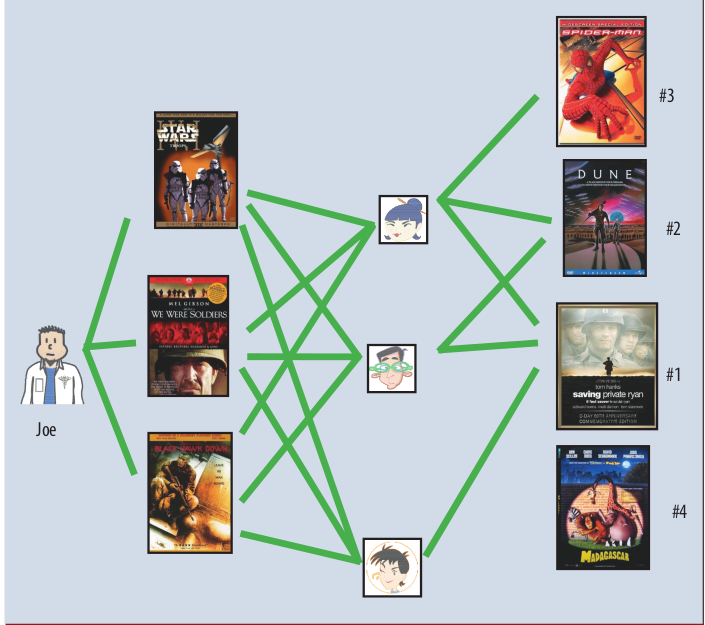
\includegraphics[scale=0.4]{colab}
\caption{Collaborative Filtering\cite{mainpaper}}
\label{chap0Fig:1}
\end{figure}

The user-oriented neighborhood method. Joe likes the three movies on the left. To make a prediction for him, the system finds similar and difficult to profile using content filter-users who also liked those movies, and then determines which other movies
ing. While generally more accurate than
they liked. In this case, all three liked Saving Private Ryan, so that is the first
content-based techniques, collaborative
recommendation. Two of them liked Dune, so that is next, and so on.


\subsection{Hybrid System\cite{hybrid}}
Hybrid systems means systems which are using both collaborative and content based filtering together. Hybrid systems are found to have better result than individual approaches alone.

\section{Music Playlist Generation} \label{sec1.1}
Music Playlist Generation simply means the task of generating a sequence of songs suitable for a particular user based on various inputs  given by the user. Inputs can be explicit like artist name, genre, current emotion or implicit like current time (users may like to listen to happy songs in morning) ,facial expression,etc. We have used artist name or band name as the input based on which playlist will be generated. 


\section{Music Playlist Shuffling} \label{sec1.1}
Music Playlist Shuffling means rearranging the playlist songs in such a order which is appealing to the user. It also mean changing the order dynamically based on user inputs(like whether user skipped current track or listened to the whole song or skipped in between)



\chapter{Related Reading}\label{chap1}
\section{Matrix Factorization} \label{sec1.1}
Some of the most successful realizations of latent factor models are based on matrix factorization .In its basic form,matrix factorization characterizes both items and users by vectors of factors inferred from item rating patterns.

Matrix factorization allows incorporation of additional information means when explicit features are not available then implicit features like user behaviour, search pattern, browser history can be incorporated.

\subsection{A BASIC MATRIX FACTORIZATION MODEL\cite{mainpaper}}
Matrix factorization models map both users and items
to a joint latent factor space of dimensionality f, such that
user-item interactions are modeled as inner products in
that space.

\[r_u_i = q_i^T*p_u\]
    								Equation 1

r_u_i = predicted rating by user u for item i

q_i = feature vector for item i

p_u = feature vector for user u

The major challenge is computing the mapping of each item and user to factor vectors q_i , p_u \subset R_f.


After that, rating of a item with respect to a user can easily be calculated using above equation.

This model is closely related to SVD(single value decomposition). Applying SVD in collaborative filtering domain require factoring the user-item matrix. But user-item matrix is very sparse and contain many missing elements. Conventional SVD is undefined for such a matrix. This sparse matrix is also very prone to over-fitting. 

Hence Stochastic gradient descent can be used to factorize the user-item matrix.

\subsection{ADDING BIAS}

Equation 1 can be modified to account for various bias in item popularity and user perception. Means there may be some users who tend to rate more or less than the average. The rating given by these users do not tell the actual popularity of the items. hence a bias need to be added. Also a item that in general do not suite the user but it is extremely popular currently. such items must be recommended to the user. hence a bias need to added.
\[b_u_i = \mu + b_i + b_u\]

The bias involved in rating rui is denoted by bui and accounts for the user and item effects. The overall average rating is denoted by u. The parameters bu and bi indicate the observed deviations of user u and item i, respectively,from the average.

\subsection{TEMPORAL DYNAMICS}
User perception may be changing with time means user may be used to give higher rating to items earlier but now he/she will a lower rating. Hence the bias related to this user must be dynamic(function of time).

Similarly, item popularity may also be changing with time hence bias related to this item must also be dynamics.
\[r̂ _u_i (t) = u + b_i (t) + b_u (t) + q_i p_u (t)\]


\subsection{varing confidence level}
It is possible people rating items are not very confident about their rating means same items shown to the same person can have different ratings. Hence a equation must be modified to take care of this fact also.
\[min \Sigma C (r_u_i - \mu - b_u - b_i - q_i^T p_u )^2 + λ(|| q i ||^2 + || p u ||^2
+ b_u^2 + b_i^2 )\]

\section{Predictive Music Shuffling Algorithm\cite{predictiveShuffling}}
Most music players uses a minimal randomization algorithm known as Fisher-Yates algorithm.
Fisher–Yates shuffling is similar to randomly picking numbered tickets out of a hat without replacement until there are none left.

However, this does not account for any
intuitive approach. we need a algorithm that can work according to user preference.

For example, completely random algorithm can choose the same song again and again or can choose similar song one after another but we do not want this. we want a algorithm that can determine the next song based on user preference and action such as if he/she skipped the current song then next song must be different from this one.

The following approach works on the ID3 tags of a sound track. ID3 tags include \textbf{artist, album, genre, song release date}. Based on these, 'nearness' factor of all the songs in the music library are calculated respective to the song first played by the user. The higher the value of the nearness factor, higher are its chances of being played next.The nearness factor is assigned based on 1 or 2-point increment to the default value of 0 corresponding to each matched tag of the two songs. The songs with a high value of nearness factor are played first. The nearness factor is calculated based on the weight generator algorithm. The time for which the current song is played also influences whether the ones similar to this would be played next or not

\chapter{Music Playlist Generation}\label{final}
\section{DATA SET }

\textbf{last.fm-dataset-360K}

March 2010

Version 1.2


\textbf{Dataset has two files} :-
\begin{enumerate}
\end{enumerate}

1. First file(usershal-profile.tsv) contains general information about users

	\textbf{columns} = [user , gender , age, country, signup]

2. Second file(usersha1-artmbid-artname-plays.tsv) contains information about user and artist song plays

		\textbf{columns} = [user, musicbrainz-artist-id, artist-name, plays]



\section{Dataset Preprocessing and modification}

user-profile pre-processing

\textbf{columns} = [user, country]

user-artist-plays file pre-processing

\textbf{columns} = [user, artist-name, plays]

Unpopular artist are removed and after some modification final data set

\textbf{columns} = [user, artist-name, plays, total artist plays, country]



\section{K-Nearest Neighbour\cite{code}}
We have looked at various collaborative approaches like Latent factor model and matrix factorization method. we have used KNN model on last.fm data set to form recommendation system.

Basically, KNN algorithm assumes that similar thing exist in close proximity. we have to define a distance function to find distance between two points (could be as simple as Manhattan distance or Cartesian's distance). Then using this function we find K nearest neighbour to the query point.

\textbf{Pseudo Code}

Initialize K to your chosen number of neighbors

1. For each example in the data

1.1 Calculate the distance between the query example and the current example from the data.

1.2 Add the distance and the index of the example to an ordered collection

2. Sort the ordered collection of distances and indices from smallest to largest (in ascending order) by the distances

3. Pick the first K entries from the sorted collection

4. Get the labels of the selected K entries

5. If regression, return the mean of the K labels

6. If classification, return the mode of the K labels

we have eliminated unpopular artist means only those artist are taken whose total count is greater than \textbf{popularity threshold} which is a hyper parameter. In current implementation we have kept this number to be 1,00,000. We have also taken only \textbf{American user} mainly to reduce data. This is also a hyper parameter.
Then on this reduced data, KNN model is trained.

\section{Playlist Generation}
We will generate top 100 recommendation using our music recommendation model and out of these 100, 10(These 10 will be chosen based on shuffling algorithm discussed in next chapter ) will be used as playlist. 

\begin{figure}
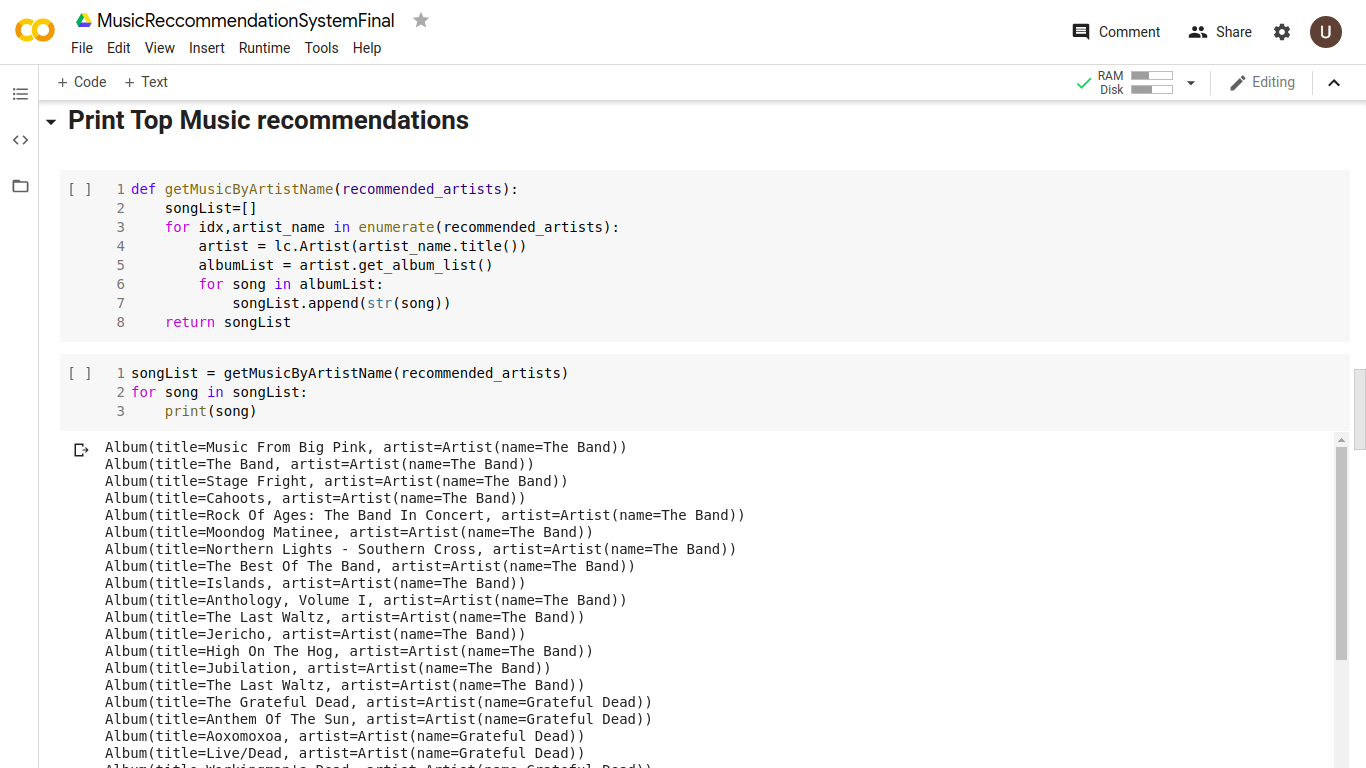
\includegraphics[scale=.8]{report/recommendedMusic.png}
\caption{Generated Playlist}
\label{chap0Fig:2}
\end{figure}
\chapter{Music Playlist Shuffling}\label{final}
Since our recommendation system runs very frequently(every hour or every day), it is necessary for the recommendation system to re-score the available items at every period of time. let's say we have a time period of T then after every time period the item list should have some changes. But in this period the user will get the same list of items. in today's time user can get bored if he/she sees the same content every time he/she opens the application during the period T.There can be many ways this scenario can happen but imagine the user opens the application and doesn't like the recommended items and is too lazy or busy to scroll or search for something else.If the user opens the application again some minutes later to find exactly the same content as before this might have a big (negative) impact on the retention for this user.

\section{Shuffling}
One solution to this problem is to shuffle the content of the playlist in such a way that it remains
relevant to the user. After shuffling, the list can have some new items but in a different order.
we can use shuffling in two ways- One is that we have a large playlist(size m) of items and we shuffle the whole playlist and show top-n out of m items.Here after every time some items can change its order and some new items can also appear in top-n list. Another way is that we can have a playlist of size n and we shuffle the whole list and show all the items of the list.Here no new item will appear but the order of the items will be changed.

Here are the types of shuffling we use

\subsection{Fisher-Yates Shuffle}

The assumption here is, we are given a function rand() that generates random number in O(1) time.The idea is to start from the last element, swap it with a randomly selected element from the whole array (including last). Now consider the array from 0 to n-2 (size reduced by 1), and repeat the process till we hit the first element.Fisher–Yates shuffle Algorithm works in O(n) time complexity.


\textbf{How does this work?}
The probability that ith element (including the last one) goes to last position is 1/n, because we randomly pick an element in first iteration.

The probability that ith element goes to second last position can be proved to be 1/n by dividing it in two cases.

\textbf{Case 1}: i = n-1 (index of last element):
The probability of last element going to second last position is = (probability that last element doesn’t stay at its original position) x (probability that the index picked in previous step is picked again so that the last element is swapped)
So the probability = ((n-1)/n) x (1/(n-1)) = 1/n

\textbf{Case 2:} 0 < i < n-1 (index of non-last):
The probability of ith element going to second position = (probability that ith element is not picked in previous iteration) x (probability that ith element is picked in this iteration)
So the probability = ((n-1)/n) x (1/(n-1)) = 1/n




\textbf{pseudo code}:

     Choose i = from last index of the list to first index of the list:
     
     choose j = Random value among 0 to ith index:
     swap(value at i th index, value at j th index

Fisher-Yates algorithm for shuffling chooses one index randomly and one index linearly from last position to first position and swap the elements of these two positions.


\begin{figure}
\centering
\begin{subfigure}
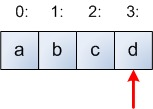
\includegraphics[scale=.5]{report/fy1.jpeg}
\label{chap3Fig:1}
\end{subfigure}
\begin{subfigure}
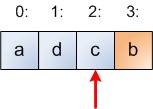
\includegraphics[scale=.5]{report/fy2.jpeg}
\end{subfigure}
\begin{subfigure}
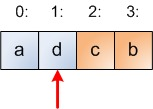
\includegraphics[scale=.5]{report/fy3.jpeg}
\end{subfigure}
\begin{subfigure}
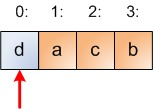
\includegraphics[scale=.5]{report/fy4.jpeg}
\end{subfigure}
\begin{subfigure}
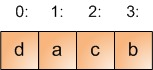
\includegraphics[scale=.5]{report/fy5.jpeg}
\caption{Fisher Yates}
\end{subfigure}
\end{figure}



\begin{figure}
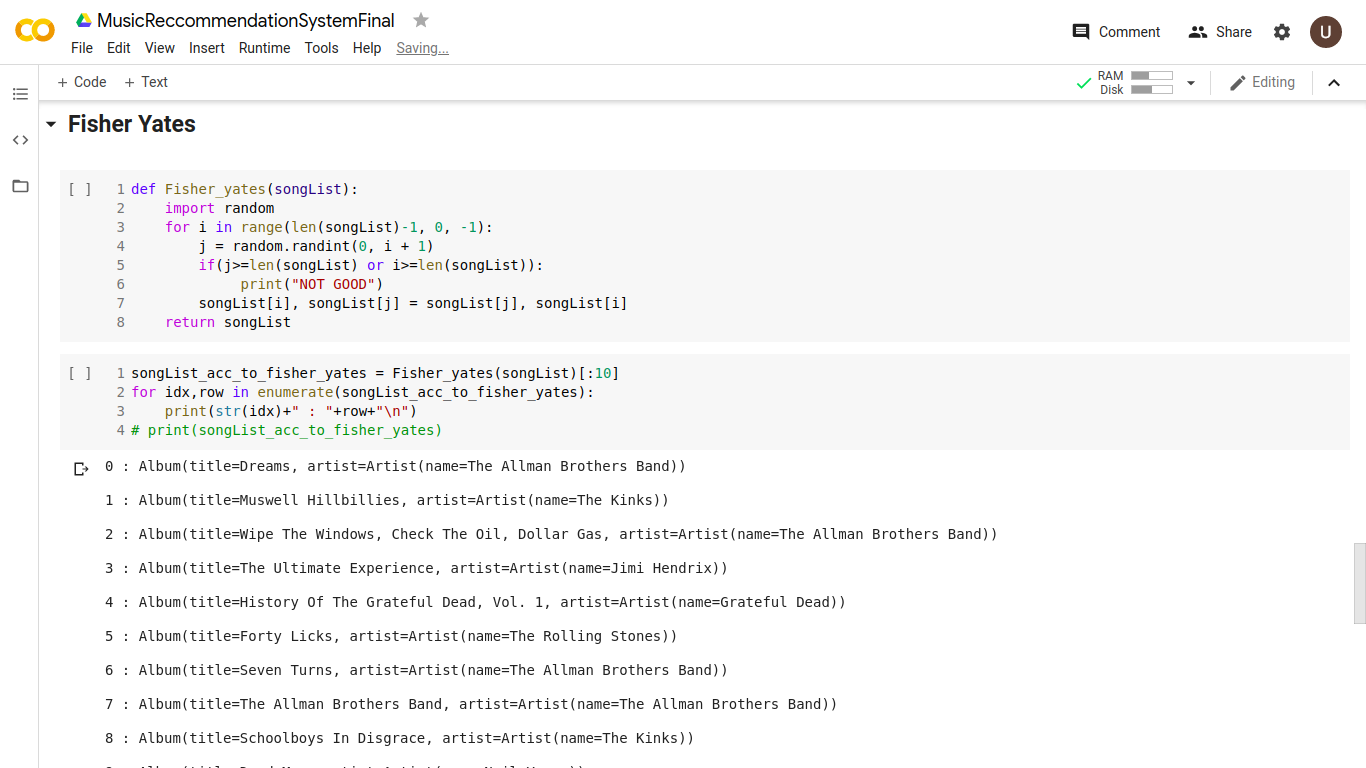
\includegraphics[scale=.5]{report/Fisheryates.png}
\caption{Flow Chart}
\label{chap0Fig:2}
\end{figure}





\subsection{Etilist Shuffle}
This is a very simple approach, In this method of shuffling, every item has given some weight then we calculate weighted probability. Items will be chosen for shuffling based on its weighted probability.

(this is the same as sampling from a multinomial distribution without replacement)

A parameter called inequality is introduced as a knob to tune the weight probability difference between positions.
maximum probability remains on the initial positions in the Etilist Shuffle, Probability decays monotonically with the distance from the initial position, higher ranked items have a higher chance of  being moved from their initial position.

\textbf{Importance of inequality:} If we want higher items to be more probable to remain on top position we'll increase inequality value.

\textbf{features: } 

1. The maximum probability remains on the initial position.

2. Probability decays monotonically with the distance from the initial position.

3. The distribution is non-symmetrical but smoother than the previous example.

4. A big win is that the inequality parameter has a direct understandable impact on the resulting distributions, want higher items to be more probable to remain on top? Increase inequality. In addition, the behavior translates into the desired functionality:

5. Top content would still be relevant after shuffle.
Content is not the same.
Some content has changed position.

\textbf{Drawback:}

The elitist shuffle function is much slower than np.random.shuffle, but still fast for a common application. Considering scenario where the items to shuffle are 100, the elitist shuffle function takes around 1.8ms.



\begin{figure}
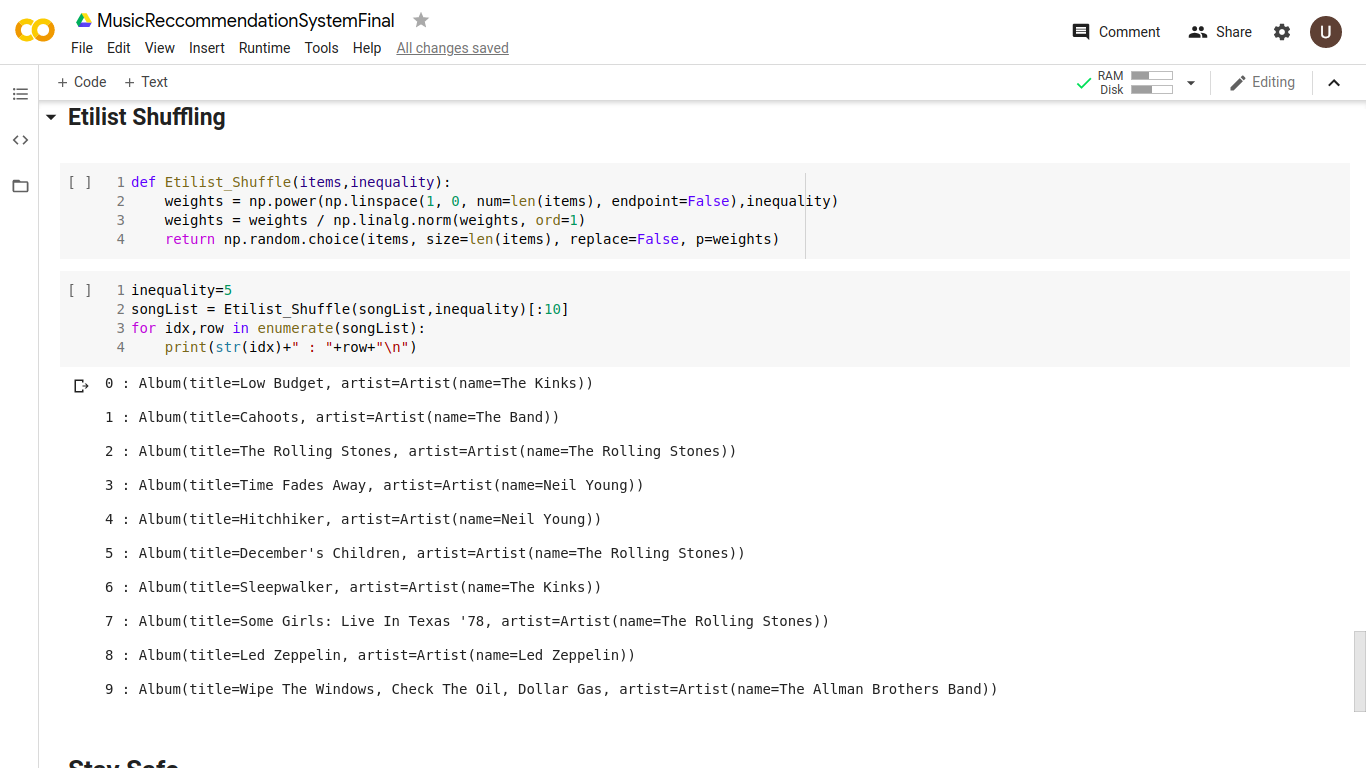
\includegraphics[scale=.5]{report/EtilistShuffing.png}
\caption{Flow Chart}
\label{chap0Fig:2}
\end{figure}



\begin{figure}
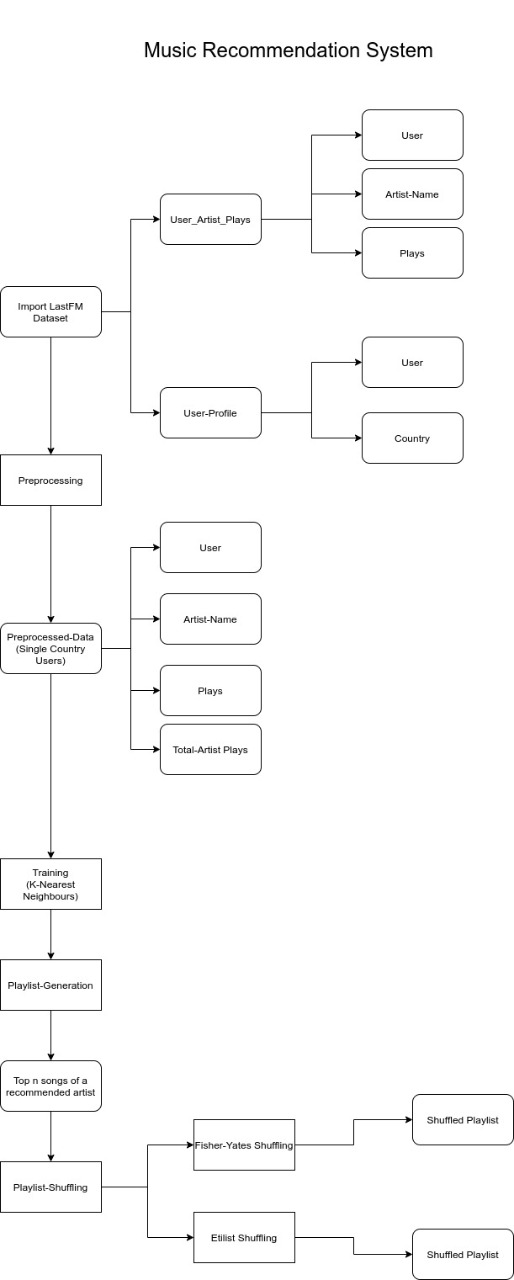
\includegraphics[scale=.5]{report/flowchar.jpeg}
\caption{Flow Chart}
\label{chap0Fig:2}
\end{figure}
\chapter{Conclusions and Discussion}\label{final}
This project implements a Music Playlist generator and shuffling algorithm based on minimum user input using KNN model and different shuffling algorithms

For Playlist generation, Top k recommended songs of music recommendation system  are used as a playlist.

For playlist Shuffling, different shuffling algorithms likeFisher Yates,EtilistShuffling are used.

\section*{Future Directions}
This report gives rise to a number of important problems and possible optimization that need to be looked into further:
\begin{itemize}

\item {For the Playlist Generation, More advanced deep leaning based algorithm can be used.}

\item {For the Playlist Shuffling, Weights can be given to songs based on features like likeness to artist,genre,etc and then some weight based shuffling algorithm can be developed.}

\item {For the Playlist Generation, More explicit features like current user mood, genre, etc can be used. we could develop algorithms that will include these features. But for this data set is not easily available.}

\item {Also, Implicit features like music history, facial expressions, current time can also be taken but again data set becomes a problem. }


 \end{itemize}


\bibliographystyle{IEEEtran}
\bibliography{report}
\end{document}
